% chapter2.tex (Chapter 2 of the thesis)

\chapter{Assessment of Harmonic Based Techniques and Repertoire}

% //TODO: Talk about Pythagoras - https://trello.com/c/uo0AALKP/1-talk-about-pythagoras
Goals for this chapter:

1. Explain sound production of stringed instruments.
2. Explain the way in which the techniques differ from standard sound production.
3. Explain the qualities of the techniques.
4. Explain the notation.



Harmonic based techniques invariably make use of the harmonic series in one way or another. 
The harmonic series is a sequence of tones in which the frequency of each is an integer multiple of the fundamental frequency. 
The earliest forms of tuning systems were based around these, but modern instruments are tuned using equal temperament. 
The pitch of sound on stringed instruments is determined via tension, effecting the speed (and consequently pitch) the string vibrates at. 
Altering the tension is most commonly achieved via fingerings on the instrument's fingerboard, but bow pressure can also play a part in pitch production (see subharmonics).

The objective categorisation of techniques is a Sisyphean task due to the variability of the techniques, but general guidelines can be made; Dick's \emph{The Other Flute} makes good use of quantifying qualitative data about the properties of multiphonics, and the idea of his tables will be used, adapting the format to each technique.\autocite[84]{dickOtherFlute1989}

To be able to pass any judgement on the techniques, we must first understand these techniques' capabilities, limitations, qualities, considerations, and values. 
Without references to other composers' works, any implication of authority on what constitutes as `idiomatic' writing is baseless. 
As such, references to other works will be used to support claims. 
Where no such references are available, it will be marked as the author's personal opinion. 
Even without any available references to substantiate compositions as idiomatic, their creation contributes to the literature, and thus can be used if not as an example, a warning on what not to do. 

\subsection{Background}
All of the techniques covered in this exegesis involve the excitation of a string instrument's string in a non-standard way. 
A small amount of understanding the physics behind these techniques is required, though they are not fully understood.
Strings create sound via the Helmholtz motion, which 

Subharmonics are perhaps a misnomer, and do not \emph{technically} fall under the branch of harmonic based techniques.
This is because their production is not by ways of the overtone (or undertone) series, as the pitches that can be produced do not follow any discernable ratio based pattern.



% Provide an overlay of the techniques and explain how they work, the general benefits and such.
% \subsection{Research statement/problem}
% Techniques are under-developed and/or under-used.

% \subsection{Aim and scope of thesis}
% Examples of use in current literature will support use-case scenarios, dearths of usage will support the fact that they are underused.

% \subsection{Significance of work}
% The production of technique and its uses.
\newpage
\section{Subharmonics}
% TODO: Explain subharmonics - https://trello.com/c/HP0b1P3h/2-explain-subharmonics
First discovered by Mari Kimura, subharmonics are a type of overpressure which produces a sound lower than the fundamental.\autocite{kimuraHowProduceSubharmonics1999} 
When the bow is drawn across the string, the drag of the bow twists the string, creating torsional oscillation. 
Under the right conditions, these can interact with the string to produce an identifiable pitch lower than the fundamental.\autocite{Subharmonics2006} 
One of the newest string techniques, subharmonics are still in their comparative infancy, and their notation has not been formalised. 

Subharmonics represent an incredible opportunity for solo string repertoire. 
On higher pitched instruments, their use can provide harmonic support (particularly in cadenza passages) and extend the range of the instrument. 
On lower pitched instruments, subharmonics function better as a timbral mechanic, much like overpressure. 




\subsection{Subharmonics in the literature}

There have been several different ways of notating them, each with their advantages and disadvantages.
% TODO: Find pieces using subharmonics - https://trello.com/c/o0tMOEza/3-find-pieces-using-subharmonics



Possibly the first person to make use of the technique, Crumb described what we know as subharmonics as `pedal tones'.\autocite{crumbBlackAngelsImages1971} 
The use of square noteheads and a separate stave for the resultant pitch makes the technique clear and readily understandable.
\begin{figure}
    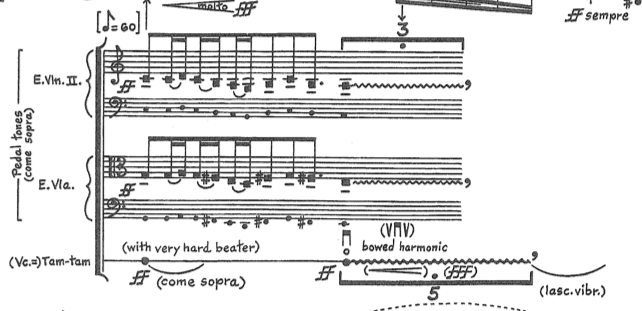
\includegraphics[width=\linewidth]{./resources/crumbBlackAngels.png}
    \caption{Excerpt from Crumb's \emph{Black Angels}.}
\label{fig:Excerpt from Crumb's Black Angels}\autocite[]{crumbBlackAngels1995}
  \end{figure}
% TODO: Citation is needed for Crumb - https://trello.com/c/Rpypkzbm/4-citation-needed-for-crumb
% TODO: Citation needed for pedal tones - https://trello.com/c/03arTJkS/5-citation-needed-for-pedal-tones

\begin{figure}
    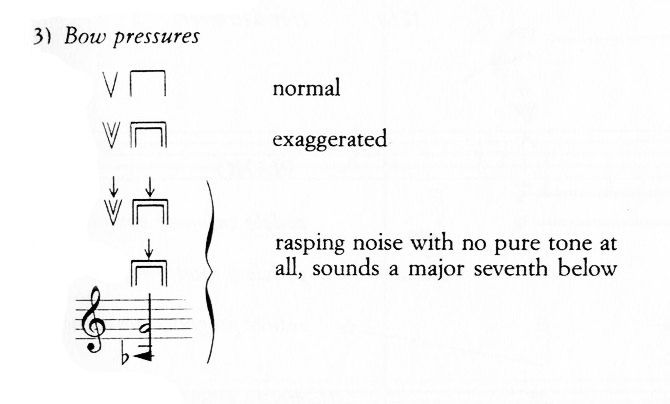
\includegraphics[width=\linewidth]{./resources/griseyVortexTemporum.jpg}
    \caption{Excerpt from Grisey's playing instructions for \emph{Vortex Temporum}.}
\label{fig:Excerpt from Grisey's playing instructions for Vortex Temporum}\autocite[]{griseyVortexTemporum}
  \end{figure}


Gerard Grisey's \emph{Vortex Temporum} features overpressure, with a subharmonic of specifically a seventh. 
Somewhat abstracted out, this hides the intended effect behind symbols, and is slower to sight read.

\begin{figure}
    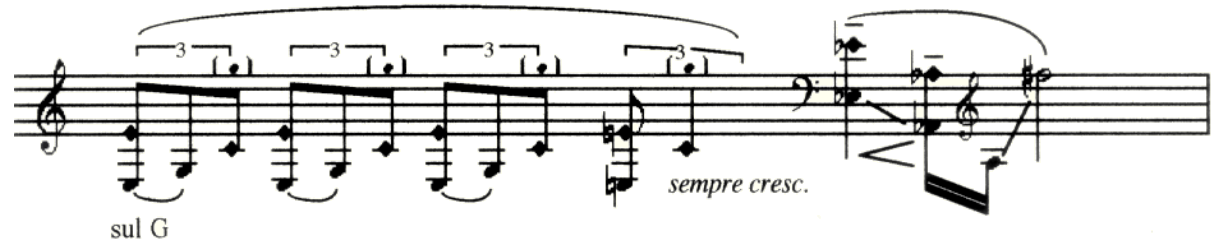
\includegraphics[width=\linewidth]{./resources/kimura_gemini.png}
    \caption{Excerpt from Kimura's \emph{Gemini}.}
\label{fig:Excerpt from Kimura's Gemini}\autocite[]{kimuraGemini1992}
  \end{figure}
  % TODO: Citation needed for Gemini

  Mari Kimura's \emph{Gemini} is an example of idiomatic usage of subharmonics on the violin. 
  Kimura's notation practice of using a harmonic denoting the intended pitch below the fundamental is similar to the standard notation of harmonics, which Gould states is to `write harmonics as the player will finger them.'\autocite[413]{gouldBars2011} 
  Unfortunately, this method proved somewhat counterintuitive in practice, as the notation was too similar, and caused sight reading issues.

  Botting notes that experimentations with octavic subharmonics yielded a pitch slightly flatter than an octave. He states \begin{quotation}
    `I developed a left hand finger technique whereby I rotate my hand slightly clockwise, pivoting on the finger stopping the string, which has the effect of sharpening the subharmonic enough to be more in tune with the fundamental.'\autocite[111]{bottingDevelopingPersonalVocabulary2019}
\end{quotation}

\subsection{Notation of Subharmonics}

The example used on Long's website, \emph{The Modern Double Bass} features a square notehead with the intended sound at pitch in a bracketed notehead, with harmonics and a technique line of `S.H'.\autocite[]{longSubharmonics2019}
It is the author's opinion that this is somewhat redundant, as just square noteheads with the intended produced pitch would be enough to delineate the technique. 
The technique line is supernumerary, and it would only be advisable to use it in extended passages of uninterrupted subharmonics.

Notationally, the best practice appears to be following Crumb's approach, condensing into one stave where possible. 


\begin{figure}
  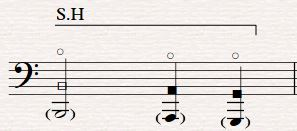
\includegraphics[width=\linewidth]{./resources/longSubharmonicNotation.jpg}
  \caption{Notation of subharmonics from Long's website, The Modern Double Bass.}
\label{fig:Notation of subharmonics from Long's website, The Modern Double Bass}\autocite[]{longSubharmonics2019}
\end{figure}

Musicians are better at sight reading above the stave than below the stave, so unlike natural harmonics, the need to split into another stave to show the resultant pitch is likely to be more common for composers wishing to use subharmonics. 
The notation of subharmonics is explored in my works \emph{The Veldt}, and \emph{Doppelganger}.


% TODO: undefined - https://trello.com/c/SU5ZEEmJ/6-- Do I need a citation for "musicians are better at sight reading above the stave than below"?
\newpage
\section{Multiphonics}
% TODO: Explain multiphonics - https://trello.com/c/6vkcY6CO/7-explain-multiphonics

Multiphonics are most commonly the domain of wind, and occasionally brass instruments, but they are an emerging technique in string writing. 
They are produced when fingerings split the string between two natural harmonics, allowing for the string to resonate at multiple frequencies.
% TODO: Citation needed for explanation of physics of multiphonics - https://trello.com/c/EboMHDaN/8-citation-needed-for-explanation-of-physics-of-multiphonics
Multiphonics on stringed instruments are difficult, but with appropriate preparation and notation, are feasible. 
Production of multiphonics, as with wind instruments, is not guaranteed, and can be dependant on a variety of external factors, including the humidity, make of the instrument, bow used, and other variables that are outside of the control of a composer. 
% TODO: Citation needed for the factors leading to multiphonics - https://trello.com/c/9iC7EAXb/24-citation-needed-for-the-factors-leading-to-multiphonics

Multiphonics are fragile, and require much preparation to execute reliably. 
Despite this, they can be used to achieve harmonies that are not otherwise achieveable through double-stopping, and lend themselves well to drawn out or slow passages of music. 
Multiphonics' exact pitching makes them ideal for music that uses ratios, microtones, or tone rows. 

\subsection{Multiphonics in the literature}

Fallowfield explores multiphonic production on the cello in her thesis CelloMap comprehensively, with video recordings of all possible multiphonics and permutations, including pizzicati.\autocite{fallowfieldCelloMapHandbook2009} 
These are isolated, though, and give little indication to the difficulty of the multiphonics.

Ashley John Long's `The Modern Double Bass' website serves a similar purpose as Fallowfield's CelloMap for the double bass\autocite{longModernDoubleBass}. 
He divides them into different categories as detailed below, some of which have more information and detail than others. 
Despite the varying degrees of detail, his work on cataloguing multiphonics is more in depth than many other resources.

\begin{table}[]
  \centering
  \resizebox{\textwidth}{!}{%
  \begin{tabular}{@{}ll@{}}
  \toprule
  \textbf{Type}                                      & \textbf{Description}                                                       \\ \midrule
  `Natural' multiphonics                             & Chart of different fingerings, similar to Fallowfield.                     \\ \midrule
  Pizzicato multiphonics                             & Description of technique, production, and result.                          \\ \midrule
  Textural multiphonics                              & Description of technique, production, result, and considerations.          \\ \midrule
  Multiphonics behind the bridge                     & Description of technique.                                                  \\ \midrule
  Artificial multiphonics                            & Chart of different fingerings, similar to Fallowfield.                     \\ \midrule
  Percussive multiphonics                            & Description of technique, production, result, and considerations.          \\ \midrule
  Timbral multiphonics                               & Description of technique.                                                  \\ \midrule
  Transformative multiphonics                        & Description and production of technique                                    \\ \midrule
  Multiphonics through Variations in Finger Pressure & Description of technique, production, result, considerations, and example. \\ \bottomrule
  \end{tabular}%
  }
  \end{table}




\subsection{Notation of Multiphonics}

Buene uses a chart of diamond noteheads with their corresponding intended multiphonic in the score for his \emph{Blacklight}.
It mimics Fallowfield's charts of corresponding nearby quartertones, though the diamond notehead is already used for harmonics, which has the potential to cause confusion.
\begin{figure}
  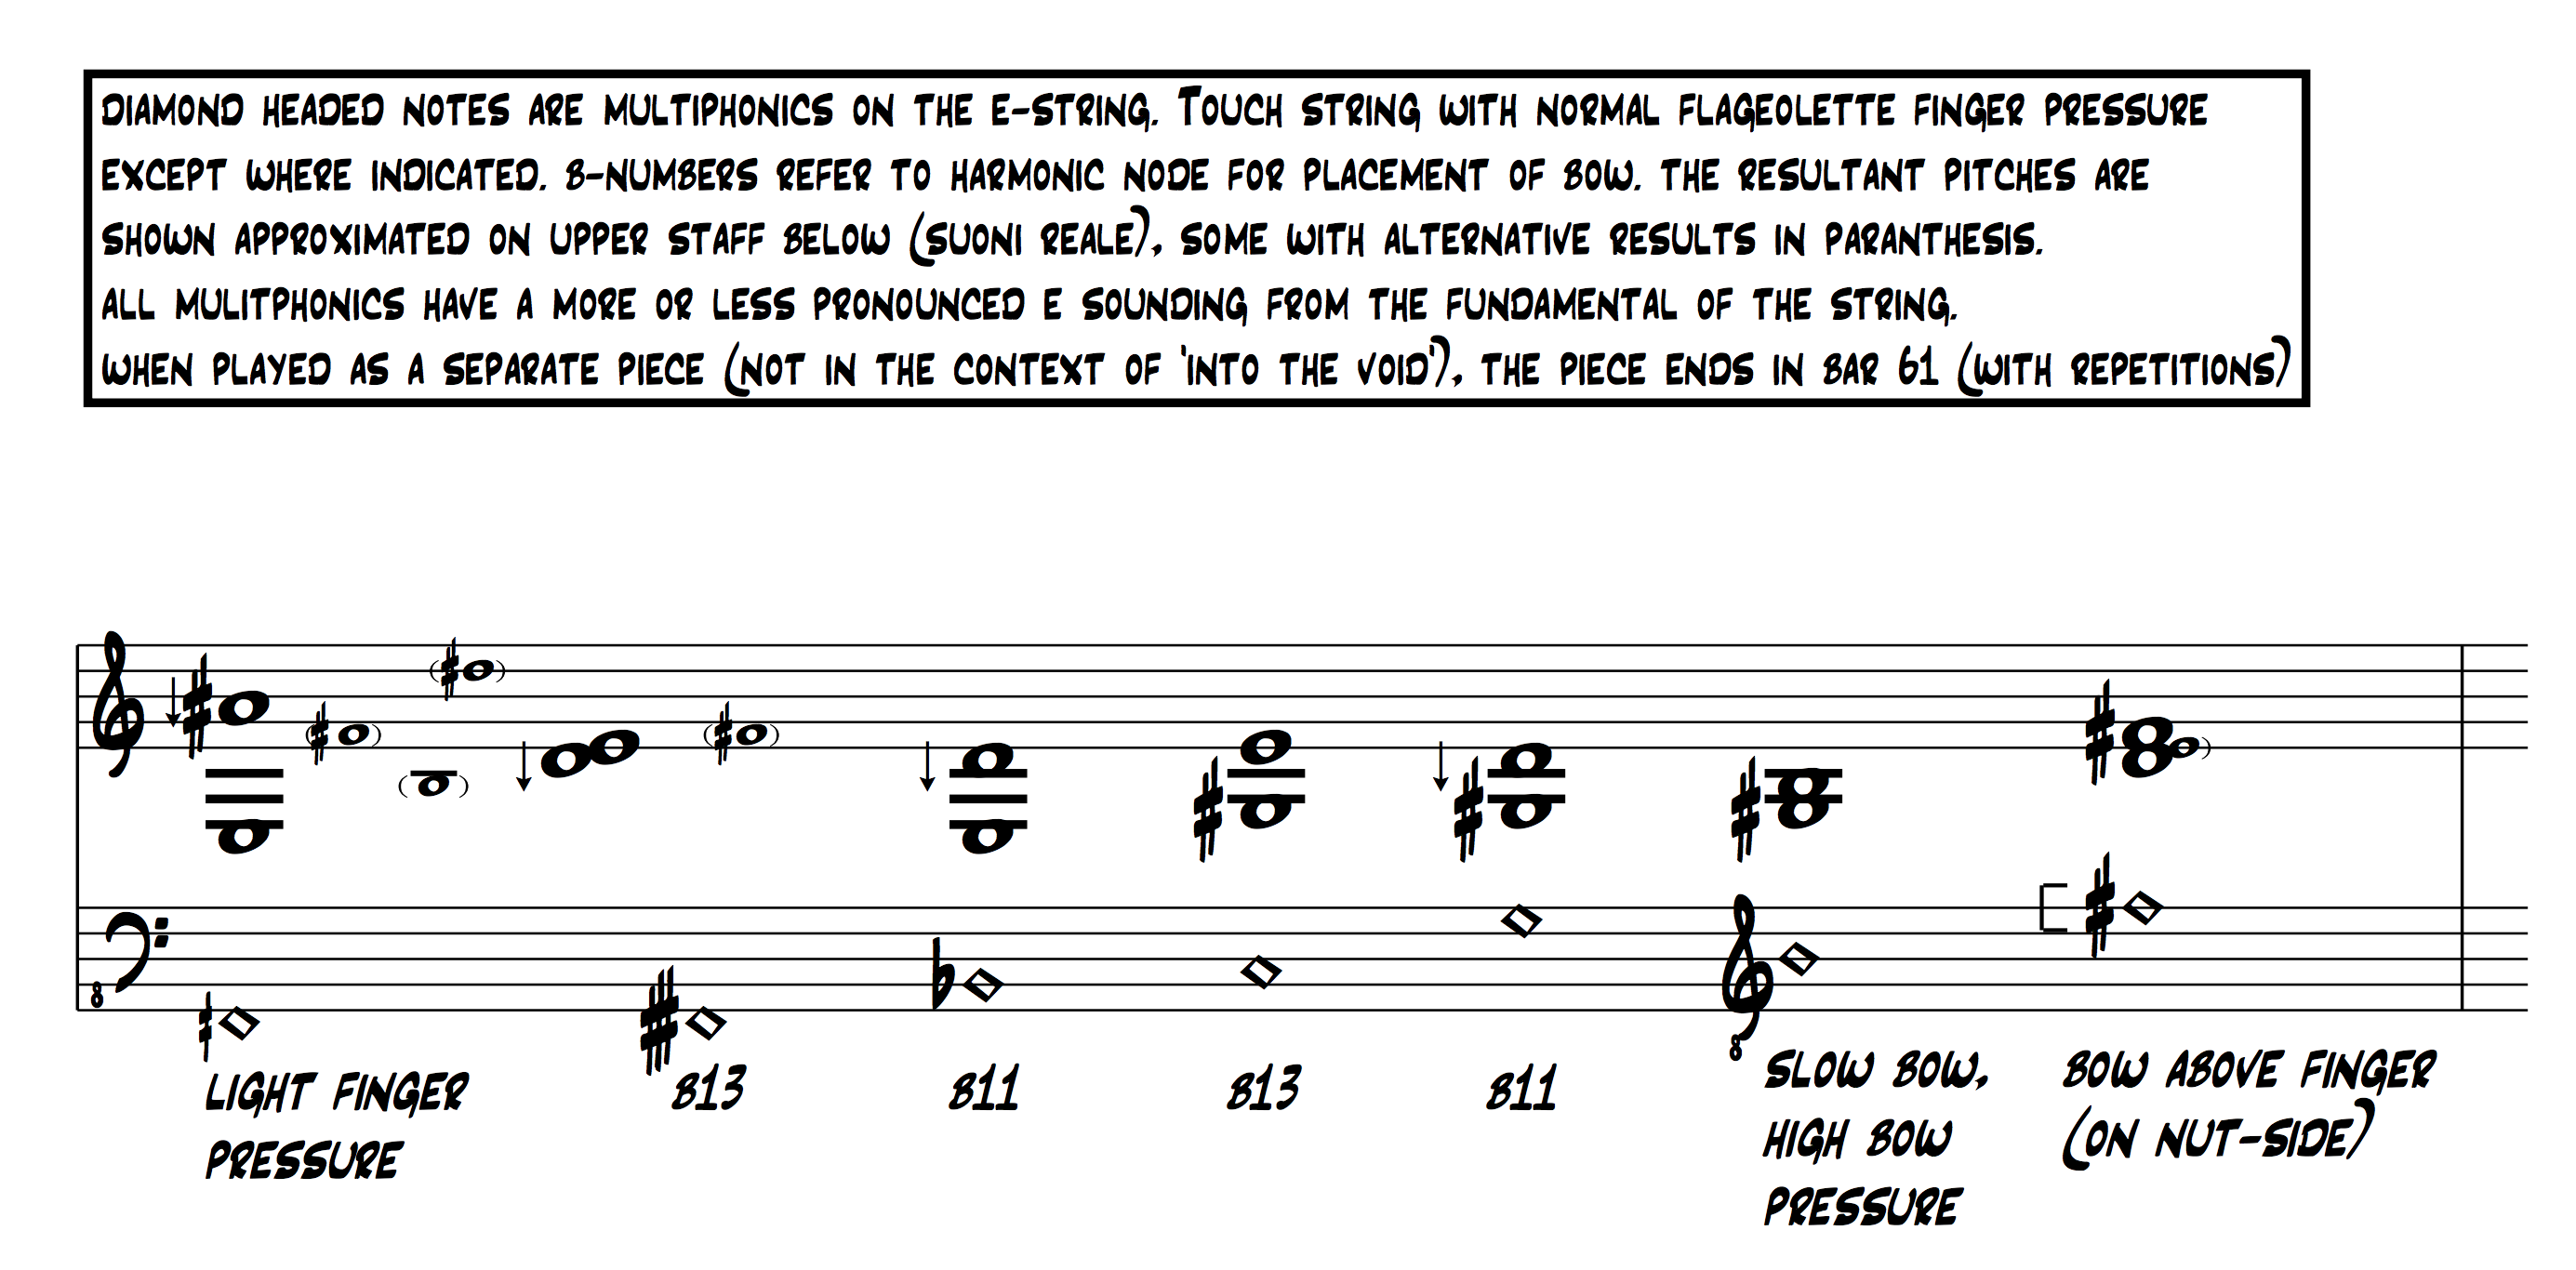
\includegraphics[width=\linewidth]{./resources/bueneMultiphonicNotation.png}
  \caption{Excerpt from Buene's Blacklight.}
\label{fig:Excerpt from Buene's Blacklight}
\end{figure}

Thelin's thesis on double bass multiphonics states:
\begin{quotation}
    `Multiphonics is [sic] always notated with the harmonic diamond sign, in tablature notation
indicating finger positions rather than musical pitches. I suggest using the symbol M. above or
below the note to indicate that it is a multiphonic sound, together with the indication on which
string to play the note (in Roman numerals).'\autocite[6]{thelinMultiphonicsDoubleBass2011}
\end{quotation}

\begin{figure}
    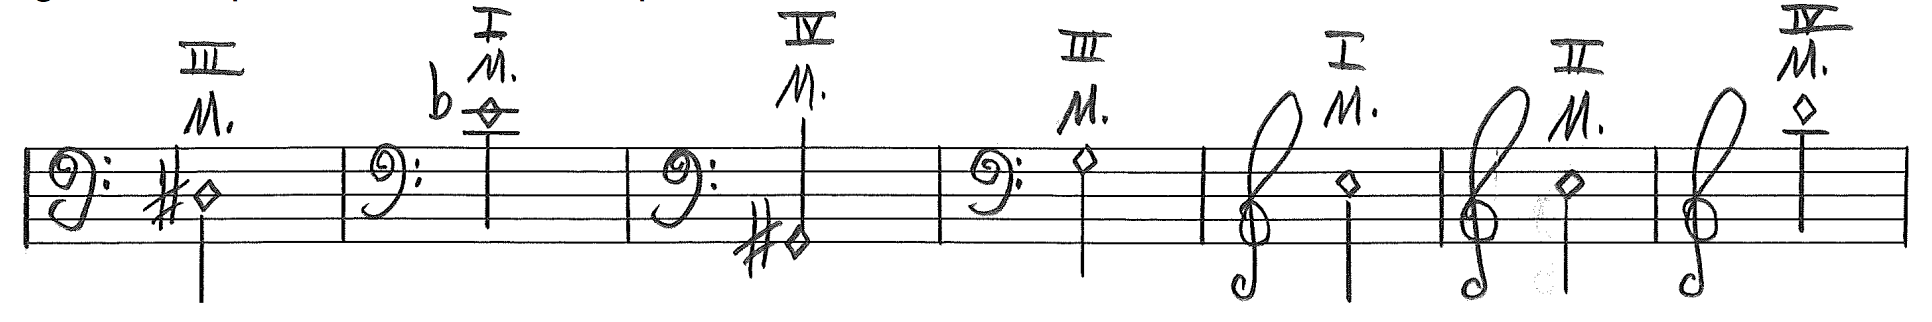
\includegraphics[width=\linewidth]{./resources/thelinMultiphonicNotation.png}
    % TODO: What is an excerpt from a thesis called? - https://trello.com/c/6xHaco1o/10-what-is-an-excerpt-from-a-thesis-called
    \caption{Excerpt from Thelin's thesis.}
  \label{fig:Excerpt from Thelin's thesis}
  \end{figure}
%   TODO: Reword Fallowfield dual harmonic positions
His notation suggestion is a somewhat less sophisticated version of Fallowfield's suggestion to notate the approximate pitch down to the cent necessary to produce the multiphonic. 
Due to the symmetry of the production of harmonics on the string, Fallowfield specifies both upper and lower positions necessary to produce the same multiphonic.\autocite[index/the-string/multiphonics-and-other-multiple-sounds/fingeringcharts.html]{fallowfieldCelloMap}
\begin{figure}
    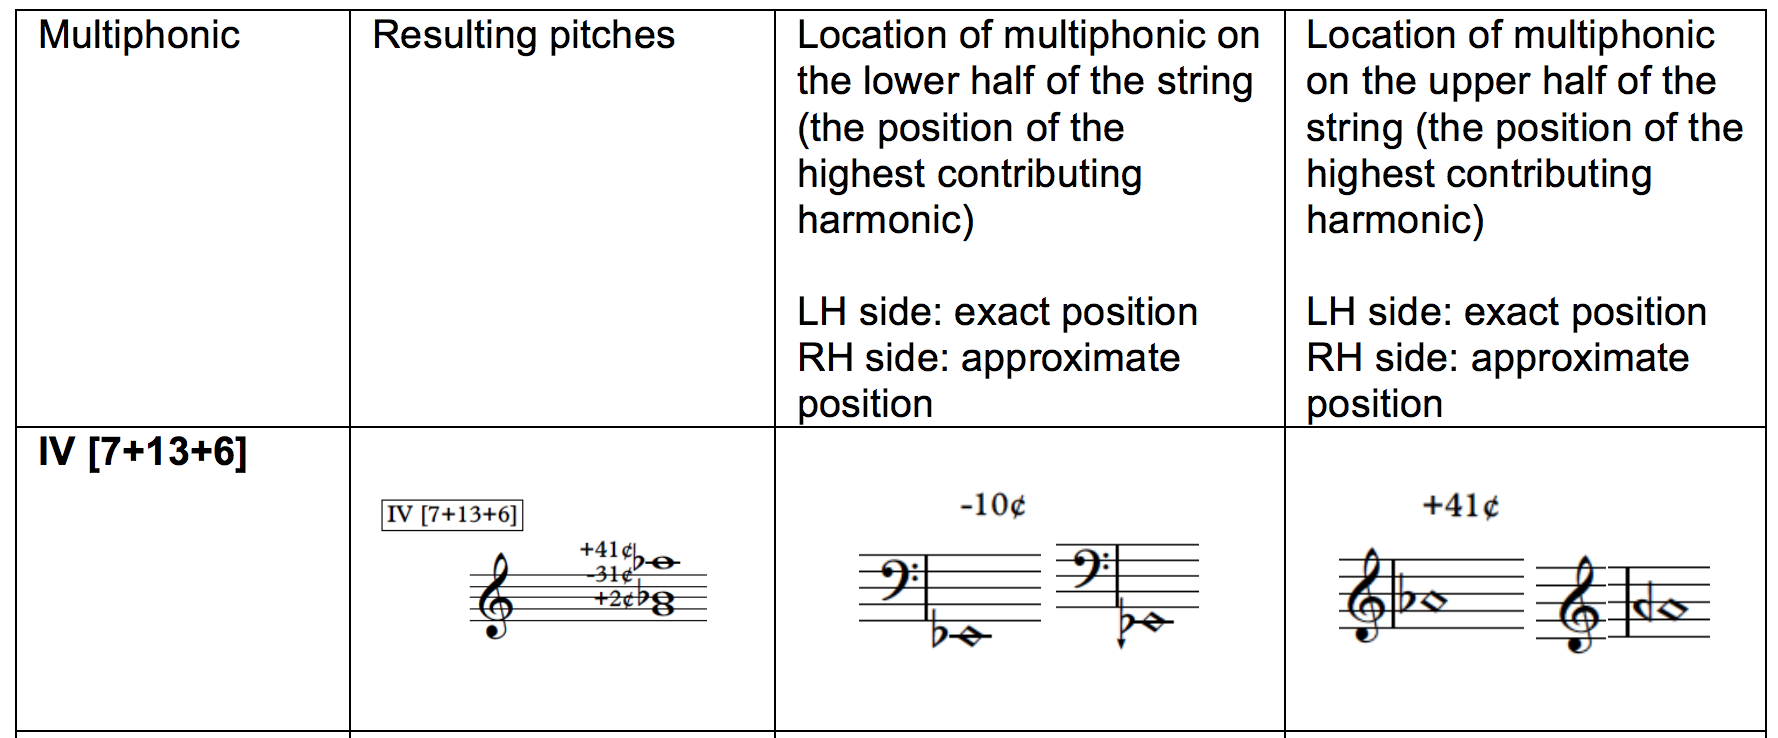
\includegraphics[width=\linewidth]{./resources/fallowfieldMultiphonicFingering.png}
    % TODO: What is an excerpt from a website called? - https://trello.com/c/04ESsMtJ/9-what-is-an-excerpt-from-a-website-called
    \caption{Excerpt from Fallowfields's website.\autocite[]{fallowfieldCelloMap}}
\label{fig:Excerpt from Fallowfields's website}
  \end{figure}

  We can see this in practice in Oliver Thurley's work for solo contrabass, \emph{yet another example of the porousness of certain borders}, where he adds another stave showing the intended pitches to be produced.\autocite{thurleyAnotherExamplePorousness2014}

  \begin{figure}
    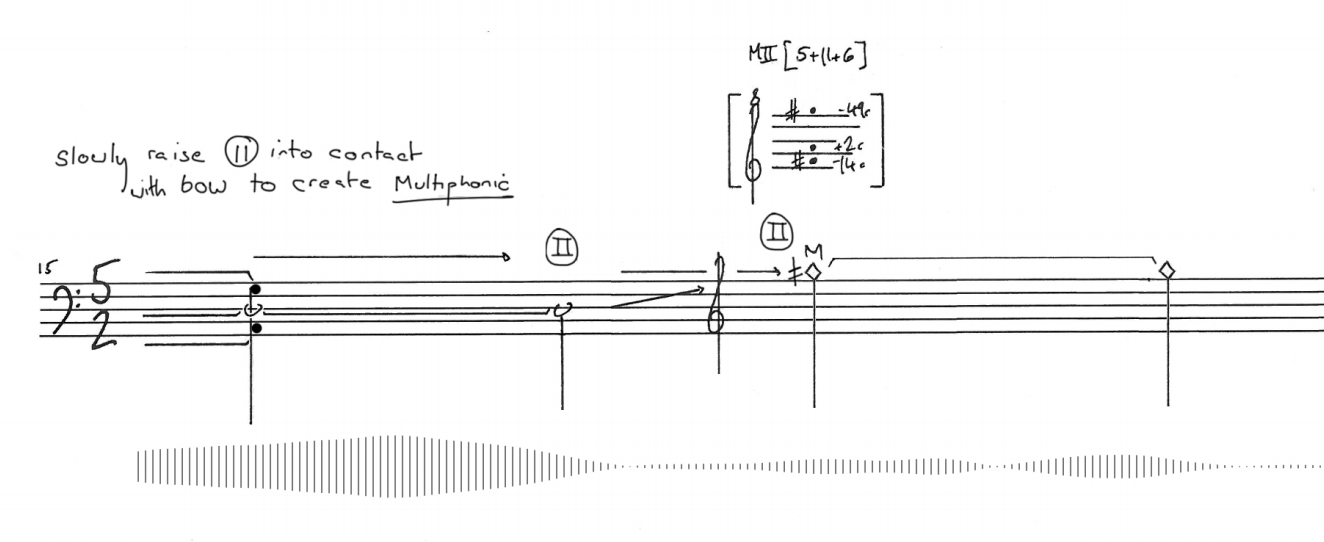
\includegraphics[width=\linewidth]{./resources/thurleyMultiphonicNotation.png}
    % TODO: What is an excerpt from a piece called? - https://trello.com/c/E9QqxFt0/12-what-is-an-excerpt-from-a-piece-called
    % TODO: Quotation marks in figure labels? - https://trello.com/c/HLJwnAwa/11-quotation-marks-in-figure-labels
    \caption{Excerpt from Thurley's \emph{yet another example of the porousness of certain borders}.\autocite[]{thurleyAnotherExamplePorousness2014}}
\label{fig:Excerpt from Thurley's `yet another example of the porousness of certain borders'}
  \end{figure}

\newpage
\section{Half-Harmonics}
% TODO: Explain half-harmonics - https://trello.com/c/0v3lKvmZ/25-explain-half-harmonics
Half-harmonics is a term assigned to the fingering pressure found somewhere in between a regular note and harmonic. 
The technique is not difficult to produce, and the resultant sound is not dissimilar to the fragility of a multiphonic, producing both the fundamental pitch, and the harmonic. 
It should be noted that the half-harmonic is a modifying left-hand technique; it can be applied to multiphonics (although the resultant sound would likely be more noise than discernably either of the two techniques), but is not compatible with subharmonics due to the bow pressure needed to produce subharmonics eliminating the possibility of half-harmonics being produced.
The terminology is not formalised, and is perhaps 

\subsection{Half-harmonics in the literature}
Half-harmonics are notably absent from the literature, with the most notable work being Sciarrino's 6 Caprices for solo violin.\autocite{sciarrinoCapricciViolino1976} 
Lachenmann also makes use of them, and states it is
\begin{quotation}
  [\dots] `important not to produce any harmonics here; the result should be a veiled, almost immaterial and hardly perceptible coloring of the dominating string sound produced by the stopped note'\autocite[foreword]{lachenmannMusikFurStreichquartett1972}
\end{quotation}
% Half-harmonics are used typically as a colourant, rather than a feature technique, and 

\subsection{Notation of half-harmonics}
Perhaps the most straight-forward technique covered in this exegesis, notation for half-harmonics have just a single variable of finger pressure to convey in notation.
The use of standard notation, modified to reflect the idea that the technique fits in 'half way between' two well established techniques (normale and harmonics) would be ideal, conforming to Gould's ideology of maintaining uniformity.
% TODO: Add Gould reference for creating new notation - https://trello.com/c/pAR2S6wg/26-add-gould-reference-for-creating-new-notation